% Options for packages loaded elsewhere
\PassOptionsToPackage{unicode}{hyperref}
\PassOptionsToPackage{hyphens}{url}
%
\documentclass[
  ignorenonframetext,
]{beamer}
\usepackage{pgfpages}
\setbeamertemplate{caption}[numbered]
\setbeamertemplate{caption label separator}{: }
\setbeamercolor{caption name}{fg=normal text.fg}
\beamertemplatenavigationsymbolsempty
% Prevent slide breaks in the middle of a paragraph
\widowpenalties 1 10000
\raggedbottom
\setbeamertemplate{part page}{
  \centering
  \begin{beamercolorbox}[sep=16pt,center]{part title}
    \usebeamerfont{part title}\insertpart\par
  \end{beamercolorbox}
}
\setbeamertemplate{section page}{
  \centering
  \begin{beamercolorbox}[sep=12pt,center]{part title}
    \usebeamerfont{section title}\insertsection\par
  \end{beamercolorbox}
}
\setbeamertemplate{subsection page}{
  \centering
  \begin{beamercolorbox}[sep=8pt,center]{part title}
    \usebeamerfont{subsection title}\insertsubsection\par
  \end{beamercolorbox}
}
\AtBeginPart{
  \frame{\partpage}
}
\AtBeginSection{
  \ifbibliography
  \else
    \frame{\sectionpage}
  \fi
}
\AtBeginSubsection{
  \frame{\subsectionpage}
}
\usepackage{amsmath,amssymb}
\usepackage{lmodern}
\usepackage{iftex}
\ifPDFTeX
  \usepackage[T1]{fontenc}
  \usepackage[utf8]{inputenc}
  \usepackage{textcomp} % provide euro and other symbols
\else % if luatex or xetex
  \usepackage{unicode-math}
  \defaultfontfeatures{Scale=MatchLowercase}
  \defaultfontfeatures[\rmfamily]{Ligatures=TeX,Scale=1}
\fi
% Use upquote if available, for straight quotes in verbatim environments
\IfFileExists{upquote.sty}{\usepackage{upquote}}{}
\IfFileExists{microtype.sty}{% use microtype if available
  \usepackage[]{microtype}
  \UseMicrotypeSet[protrusion]{basicmath} % disable protrusion for tt fonts
}{}
\makeatletter
\@ifundefined{KOMAClassName}{% if non-KOMA class
  \IfFileExists{parskip.sty}{%
    \usepackage{parskip}
  }{% else
    \setlength{\parindent}{0pt}
    \setlength{\parskip}{6pt plus 2pt minus 1pt}}
}{% if KOMA class
  \KOMAoptions{parskip=half}}
\makeatother
\usepackage{xcolor}
\newif\ifbibliography
\usepackage{longtable,booktabs,array}
\usepackage{calc} % for calculating minipage widths
\usepackage{caption}
% Make caption package work with longtable
\makeatletter
\def\fnum@table{\tablename~\thetable}
\makeatother
\usepackage{graphicx}
\makeatletter
\def\maxwidth{\ifdim\Gin@nat@width>\linewidth\linewidth\else\Gin@nat@width\fi}
\def\maxheight{\ifdim\Gin@nat@height>\textheight\textheight\else\Gin@nat@height\fi}
\makeatother
% Scale images if necessary, so that they will not overflow the page
% margins by default, and it is still possible to overwrite the defaults
% using explicit options in \includegraphics[width, height, ...]{}
\setkeys{Gin}{width=\maxwidth,height=\maxheight,keepaspectratio}
% Set default figure placement to htbp
\makeatletter
\def\fps@figure{htbp}
\makeatother
\setlength{\emergencystretch}{3em} % prevent overfull lines
\providecommand{\tightlist}{%
  \setlength{\itemsep}{0pt}\setlength{\parskip}{0pt}}
\setcounter{secnumdepth}{-\maxdimen} % remove section numbering
\ifLuaTeX
  \usepackage{selnolig}  % disable illegal ligatures
\fi
\IfFileExists{bookmark.sty}{\usepackage{bookmark}}{\usepackage{hyperref}}
\IfFileExists{xurl.sty}{\usepackage{xurl}}{} % add URL line breaks if available
\urlstyle{same} % disable monospaced font for URLs
\hypersetup{
  hidelinks,
  pdfcreator={LaTeX via pandoc}}

\author{}
\date{}

\begin{document}

\hypertarget{logistic-regression}{%
\subsection{Logistic Regression}\label{logistic-regression}}

\begin{frame}{The logistic model}
\protect\hypertarget{the-logistic-model}{}
The log-odds of an event increase linearly with an independent variable.

\[
\log\frac{p}{1-p} = ax+b
\]

\textbf{Example:} The chance that a person buys a product depends on how
many times they encounter advertising for that product.
\end{frame}

\begin{frame}{The sigmoid function}
\protect\hypertarget{the-sigmoid-function}{}
\[
\log\frac{p}{1-p}=ax+b
\]

means that

\[
p(x)=\frac{1}{1+e^{-ax-b}}
\]
\end{frame}

\begin{frame}{The logistic curve}
\protect\hypertarget{the-logistic-curve}{}
The function

\[
\sigma(x)=\frac{1}{1+e^{-x}}
\]

is called the logistic function.

\begin{figure}
\centering
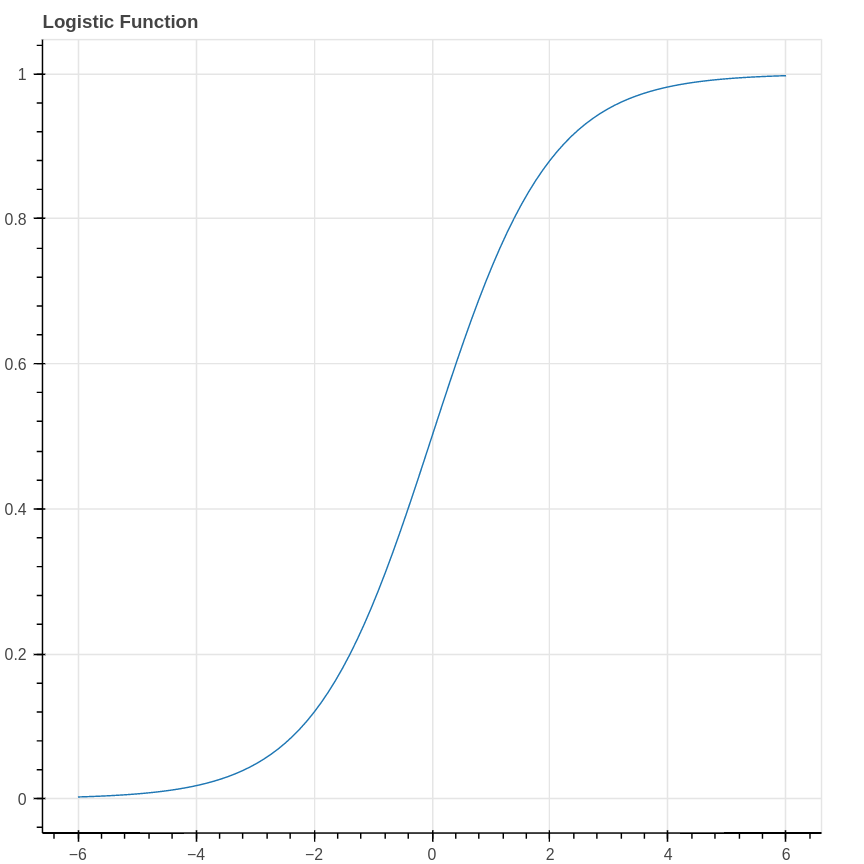
\includegraphics[width=0.5\textwidth,height=\textheight]{logistic_curve.png}
\caption{Logistic Curve}
\end{figure}
\end{frame}

\begin{frame}{Sample data}
\protect\hypertarget{sample-data}{}
Likelihood of event increases with \(x\). Out of 100 tries:

\begin{longtable}[]{@{}llllllll@{}}
\toprule()
\(x\) & -3 & -2 & -1 & 0 & 1 & 2 & 3 \\
\midrule()
\endhead
Occurrences (out of 100) & 10 & 18 & 38 & 50 & 69 & 78 & 86 \\
\bottomrule()
\end{longtable}
\end{frame}

\begin{frame}{Two points of view}
\protect\hypertarget{two-points-of-view}{}
\begin{figure}
\centering
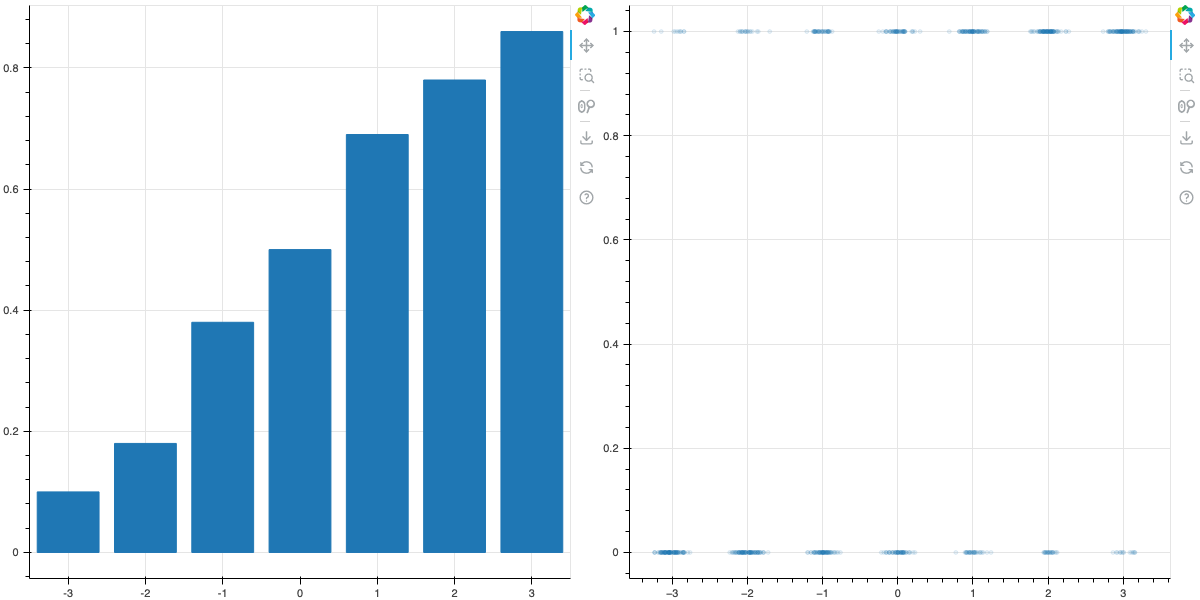
\includegraphics[width=4in,height=\textheight]{logistic_plots.png}
\caption{Logistic Data}
\end{figure}
\end{frame}

\begin{frame}{The Likelihood}
\protect\hypertarget{the-likelihood}{}
The parameters \(a\) and \(b\) are unknown. But if we knew them, then we
could figure out how likely our results were. For example, the chance of
getting \(10\) positive outcomes is

\[
p(10+ | x=-3, a,b) = C(\sigma(a(-3)+b)^{10}(1-\sigma(a(-3)+b))^{90}
\]

where \(C\) is a constant (it's a binomial coefficient).
\end{frame}

\begin{frame}{More on the likelihood}
\protect\hypertarget{more-on-the-likelihood}{}
Assuming independence (given \(x\), \(a\), and \(b\)) the chance of our
data is

\[
P(\mathrm{data}|a,b)=C P(10+|x=-3)P(18+|x=-2)\cdots P(86+|x=3)
\]
\end{frame}

\begin{frame}{Still more}
\protect\hypertarget{still-more}{}
Here each term is

\[
P(y+|x)=\sigma(ax+b)^{y}(1-\sigma(ax+b)^{N(x)-y}
\]

where \(N(x)\) is the number of trials with that given \(x\) value.
(this is a Binomial random variable).
\end{frame}

\begin{frame}{The log likelihood}
\protect\hypertarget{the-log-likelihood}{}
We want to find the \(a\) and \(b\) that make our observed data
\emph{most likely}. To do this we need to find \(a,b\) that maximize
\(P\) or, more simply \(\log P\).

\[
\log P = \sum_{i=0}^{6} \left[ y_{i}\log P(y_{i}|x_{i}) + (100-y_{i})\log(1-p(y_{i}|x_{i}))\right]
\]

We can drop the constant since it won't affect where the maximum occurs.
\end{frame}

\begin{frame}{Vector/Regression Form}
\protect\hypertarget{vectorregression-form}{}
Our data matrix consists of \(N\) rows (and 1 column), one for each
person viewing the ads. The entry in each row is the number of times
they saw the add.

The target matrix consists of 0 and 1 depending on whether they made a
purchase or not.

We want to ``fit'' an equation that gives \(0\) or \(1\) as a function
of \(x\), but we can't do this exactly, only in probabilistic terms.

This is why it's called ``regression.''
\end{frame}

\begin{frame}{More on Vector/Regression Form}
\protect\hypertarget{more-on-vectorregression-form}{}
For each row of our matrix, the chance that \(y_i\) is \(1\) is
\(p(x_i)\) (given by the sigmoid function with parameters \(a\), \(b\))
and the chance that \(y_i=0\) is \((1-p(x_i))\). So our likelihood is

\[
L(a,b) = C \prod_{i=0}^{N-1} p(x_i)^{y_{i}}(1-p(x_i))^{(1-y_i)}
\]

and

\[
\log L(a,b) = C'+\prod_{i=1}^{N-1} y_{i} \log p(x_i) + (1-y_{i})\log(1-p(x_i)).
\]

Ignoring irrelevant constants this is

\[
\log L = Y\cdot\log p(X) + (1-Y)\cdot\log(1-p(X))
\]

where for each row of \(X\), \(p(X)\) has \(\sigma(ax_i+b)\) with
(unknown) parameters \(a\) and \(b\).
\end{frame}

\begin{frame}{The case of multiple features}
\protect\hypertarget{the-case-of-multiple-features}{}
In the case of multiple features, we have a set of \(k\) measurements
for each sample (perhaps exposure to different types of ads) and a
single outcome (buy/do not buy). This yields an \(N\times k\) data
matrix \(X\). We seek a set of weights \(m_{1},\ldots, m_{k}\) and an
``intercept'' \(b\) so that

\[
\log\frac{p}{1-p}=\sum m_{i}x_{i}+b
\]

relates the log-odds of our event occurring with the values of the
features.

\textbf{Note:} Just as with linear regression, we can create a ``fake''
feature that is all \(1\), and then extend our data matrix to
\(N\times (k+1)\). Then \(b=m_{k+1}\) and we can write

\[
\log\frac{P}{1-P}=XM
\]

where the right side is an \(N\times 1\) matrix and the left side is an
\(N\times 1\) matrix whose entries are \(\log\frac{p}{1-p}\).
\end{frame}

\begin{frame}{The probability}
\protect\hypertarget{the-probability}{}
From this we get the matrix equation

\[
P = \sigma(XM)
\]

The matrix \(P\) has the probability of getting a positive outcome for
each sample given the features.
\end{frame}

\begin{frame}{A geometric remark}
\protect\hypertarget{a-geometric-remark}{}
One way to think of this is that if the features (a row of \(X\)),
thought of as a vector, points ``more in the direction of the weight
vector'' \(M\), then the probability of getting a positive outcome
increases. If it's perpendicular, you get even odds. If it points
oppositve the weight vector, you're unlikely to get what you want.
\end{frame}

\begin{frame}{The target}
\protect\hypertarget{the-target}{}
We have a vector \(Y\) which records when our event happened, and when
it didn't.
\end{frame}

\begin{frame}{The log-likelihood}
\protect\hypertarget{the-log-likelihood-1}{}
\[
L(M) = Y^{\intercal}\log(\sigma(XM))+(1-Y^{\intercal})(1-\log(\sigma(XM)))
\]

\textbf{Problem:} Given \(X\) and \(Y\), find \(M\) that maximizes this.
\end{frame}

\begin{frame}{Credit card default}
\protect\hypertarget{credit-card-default}{}
\begin{figure}
\centering
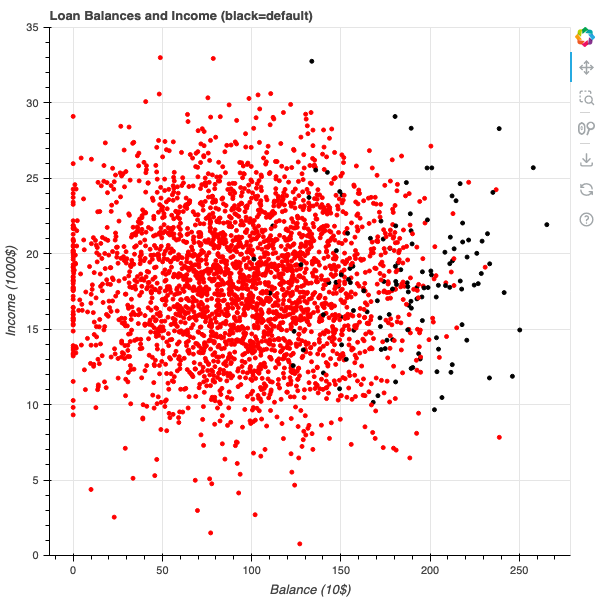
\includegraphics[width=\textwidth,height=3in]{scatter_default.png}
\caption{Default}
\end{figure}
\end{frame}

\begin{frame}{Default with logistic line}
\protect\hypertarget{default-with-logistic-line}{}
\begin{figure}
\centering
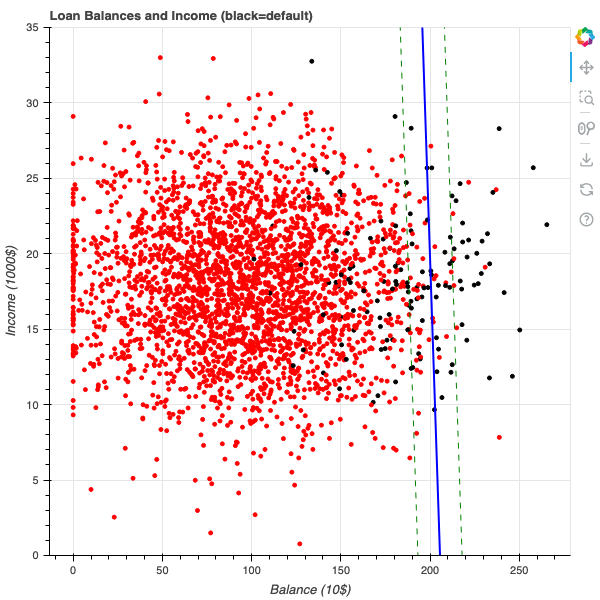
\includegraphics[width=\textwidth,height=3in]{scatter_default_with_line.png}
\caption{Default with line}
\end{figure}
\end{frame}

\begin{frame}{Logistic regression for classification}
\protect\hypertarget{logistic-regression-for-classification}{}
We can use logistic regression for classification by fitting the
logistic model and then saying that a point should be classified as
\(1\) if the probability \(p\) given by the model says it is \(1\) with
greater than \(.5\) probability.

We could also set a more stringent requirement.
\end{frame}

\begin{frame}{The ``decision surface''}
\protect\hypertarget{the-decision-surface}{}
In the logistic regression model, for a given sample \(x\) with features
\(x_{i}\) (\(i=1,\ldots, k+1\)), the log odds of that sample yielding a
``positive'' result is

\[
\log\frac{P}{1-P} = \sum x_{i}m_{i}
\]

where the \(m_{i}\) are the weights. Notice that the equation
\(f(x)=\sum x_{i}m_{i}\) is a linear function of the features. The
equation \(f(x)=0\) defines a ``hyperplane'' in feature space. (In the
graph above, this is the blue line on the default data). On that line,
it's even odds if the target is \(1\) or \(0\).

If \(f(x)>0\), the odds are better than even that the target value for
that point is \(1\); and if \(f(x)<0\) the odds are less than even.

If you are trying to classify points, you could say points where
\(f(x)>0\) should be classified as \(1\) (because, more likely than not,
the model says that they are a \(1\)).
\end{frame}

\begin{frame}{An example of classification}
\protect\hypertarget{an-example-of-classification}{}
The sklearn digits dataset consists of a large number of \(8\times 8\)
bitmap images together with labels from \(0\) to \(9\). For example:

\begin{figure}
\centering
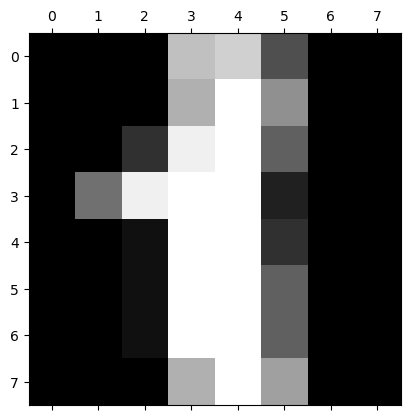
\includegraphics[width=2in,height=\textheight]{digit.png}
\caption{digit}
\end{figure}
\end{frame}

\begin{frame}{Digit recogntion (two-class)}
\protect\hypertarget{digit-recogntion-two-class}{}
We can view our images not as \(8\times 8\) arrays but as 64-entry
vectors. Let's just focus on the zeros and ones. We fit a logistic
regression model where the target is the value \(0\) or \(1\). This
turns out to do an exceptionally good job at distinguishing these
digits.
\end{frame}

\hypertarget{multiclass-logistic-regression}{%
\subsection{Multiclass logistic
regression}\label{multiclass-logistic-regression}}

\begin{frame}{Softmax}
\protect\hypertarget{softmax}{}
In multiclass logistic regression, we imagine not only that our data
depends on multiple features but that there are several possible
outcomes to our experiment.

Given numbers \(z_1,\ldots, z_n\), let

\[
F(z_1,\ldots, z_n) = \sum_{i=1}^{n} e^{z_{i}}
\]

and define the ``softmax'' function by

\[
\sigma(z_1,\ldots, z_n)=\left[\begin{matrix} \frac{e^{z_1}}{F} & \frac{e^{z_{2}}}{F} &\cdots & \frac{e^{z_{n}}}{F}\end{matrix}\right]
\]
\end{frame}

\begin{frame}{Softmax}
\protect\hypertarget{softmax-1}{}
The softmax function is the higher dimensional generalization of the
sigmoid function. Notice that it yields a vector of numbers between
\(0\) and \(1\) whose sum is \(1\).
\end{frame}

\begin{frame}{One-hot encoding}
\protect\hypertarget{one-hot-encoding}{}
The second important element of multiclass regression is how to encode
the labels. For example, in our digit problem, the labels run from \(0\)
to \(9\). Given an image, we want to compute probabilities
\(p_0,\ldots, p_9\) which add to \(1\) and, where, hopefully, the
largest \(p_i\) corresponds to the true label.

To set this up we convert our labels to one hot encoding. In this
picture, we replace our single vector with entries from \(0\) to \(9\)
with a matrix with 10 columns. Each row of this matrix has a zero
everywhere \emph{except} in the column corresponding to the label is
correct.

So if the label for an image is \(2\), the corresponding row of the
target matrix is

\[
[0,0,1,0,0,0,0,0,0,0].
\]
\end{frame}

\begin{frame}{The model}
\protect\hypertarget{the-model}{}
If we have \(N\) samples, \(k\) features, and \(r\) classes, then our
weight matrix \(M\) is \(k\times r\), our target matrix \(Y\) is
\(N\times r\), and our data matrix \(X\) is \(N\times k\). Our model
says that

\[
P = \sigma(XM)
\]

where \(\sigma(XM)\) means ``apply the softmax function to each row of
\(XM\)''; each row has \(r\) entries.

You can think of \(P\) as an attempt to ``estimate'' \(Y\).

The rows of \(P\) give the probabilities of getting each possible label
for that set of features.
\end{frame}

\begin{frame}{Max Likelihood}
\protect\hypertarget{max-likelihood}{}
As before we seek \(M\) so that the observed classification is most
likely given \(M\). To find the likelihood:

The probability that the \(i^{th}\) sample is in class \(j\) is
\(p_{s}(x_i; M)\) where \(p_{s}\) is the \(s^{th}\) entry in the
\(i^{th}\) row of the matrix \(P\). We can write this as

\[
P(i,s) = \prod_{s=1}^{r} p_{s}(x_i; M)^{y_{s}}
\]

since \(y_{s}\) is zero except at the correct class. Taking the
logarithm makes this a sum:
\end{frame}

\begin{frame}{Matrix form of max likelihood}
\protect\hypertarget{matrix-form-of-max-likelihood}{}
\[
\log P(i,s) = \sum_{s=1}^{r} y_{s}\log p_{s}(x_{i}; M).
\]

By independence, the total log probability of this data is the sum of
this over all samples and corresponding \(y\)-values.

\[
\log L(M) = \sum_{i=1}^{N} \sum_{s=1}^{r} y_{s}\log p_{s}(x_{i},M)
\]

This can be written in matrix form as

\[
\log L(M) = \mathrm{trace}(Y^{T}\log \sigma(XM)))
\]

We need to maximize this; we'll consider that later.
\end{frame}

\begin{frame}{End}
\protect\hypertarget{end}{}
\end{frame}

\end{document}
